NaturalPad est une société innovante dont le domaine d'activité est encore à ses débuts. Si les jeux vidéo sérieux commencent à être connus du grand public et leur impact reconnu, ceux pour la santé ne sont pas encore assez nombreux ni assez largement acceptés. Mon travail de stage s'inscrit en réponse à cette constatation : il s'agit de proposer une méthode de conception de jeux vidéo pour la santé qui permettrait une simplification ou une amélioration de la conception de tels jeux. Proposer plus de jeux  thérapeutiques et/ou des jeux avec un impact santé de plus grande qualité contribuerait à améliorer leur diffusion et leur reconnaissance. Pour ces raisons, il était ainsi primordial de parfaire ma connaissance des différents domaines concernés.

Cette partie présente le résultat de mes recherches, des techniques et outils existants et comporte des notions importantes à connaître pour la conception de serious games pour la santé.

	\subsection*{Méthode de travail et/ou Analyse/bilan}
Étendue sur plusieurs semaines, la réalisation de l'état de l'art était pour moi quelque chose de nouveau qui a nécessité une certaine organisation. Deux moments ont été importants : la phase de démarrage et l'arrêt des recherches. Commencer ces recherches alors que les sujets que je devais ou voulais couvrir étaient vastes et non clairement définis fut à la fois plaisant et compliqué. Bien que beaucoup de choses me semblaient intéressantes, la question était de savoir par où commencer. De la même manière, au fil de mes lectures, je découvrais de nouveaux liens et références présentant de nouveaux aspects qui eux-même renvoyaient vers d'autres solutions et articles. La difficulté était donc de juger quand mes connaissances sur un thème donné étaient suffisantes pour éviter de poursuivre d'interminables recherches, aussi intéressantes puissent elles être, le temps étant limité dans le cadre d'un stage de Master.
\paragraph{}Au niveau des lectures abordées, ma source principale fut des articles scientifiques, suivie par des articles de magazines spécialisé et articles web notamment. Pour les thèmes médicaux, un certain nombre d'articles m'a été directement conseillé par des professionnels de la santé, articles à partir desquels j'ai ensuite pu compléter mon état de l'art en suivant les références. Par ailleurs, la plupart du temps, des noms ressortent fréquemment lorsqu'on effectue des recherches sur un thème donné, ce qui permet, en plus du nombre de citations des articles, de rapidement cerner quels sont les articles et chercheurs de référénce dans le domaine.
\paragraph{}Bien entendu, afin de rendre mes lectures efficaces, je me constituais pour chacune d'elle une fiche de lecture où noter les points importants : 
\begin{itemize}
	\item Titre ou source
	\item Auteur(s)
	\item Mots clefs
	\item Synthèse
	\item Jugement personnel ou remarques
	\item Références importantes
\end{itemize}

	\subsection{Jeux Vidéo}
Durant mon stage, j'ai ainsi voulu comprendre pourquoi et comment un jeu vidéo est bon, quels en sont les mécanismes ou bien encore ce qu'est la difficulté, pourquoi et comment l'adapter.

		\subsubsection*{Population de joueurs}
Le jeu vidéo est un média récent qui trouve ses origines dans le début de la seconde moitié du XX$^{eme}$ siècle. A l'origine uniquement accessibles sur des bornes d'arcade, les jeux vidéo se sont progressivement répandus avec la sortie de consoles de salon. Selon une étude commandée par le Centre National du Cinéma et de l'image animée\href{http://www.cnc.fr}{(CNC)}, c'est près de 60\% de la population française qui jouaient à des jeux vidéo au cours de l'année 2011\cite{Cnc11}. L'âge moyen des joueurs était alors de 34,7 ans et cette population constituée de 54,1\% d'hommes fin 2011\cite{Cnc11}. L'arrivée de la console Wii et de jeux orientés plus "casuals" a permi en France une meilleure diffusion du média au sein de la population, qui accepte de plus en plus de se livrer à cette activité. Contrairement à ce que l'on pourrait croire, notamment à cause de leur méconnaissance des nouvelles technologies et du jeu vidéo plus spécifiquement, les seniors se prêtent aussi volontier à la pratique du jeu vidéo. C'est une constation que nous avons pu vérifier par nous-même lors de nos différentes sessions de tests au centre hospitalier d'Alès et dans une maison de retraite à Lille, mais aussi dans différentes lectures qui seront détaillées ci-après.
		\subsubsection*{Définition}
Le jeu vidéo est donc un média participatif en pleine extension et de plus en plus largement accepté et plébiscité par la population. \\Dans sa définition, un jeu vidéo est une extension du jeu au monde numérique en utilisant les technologies informatiques. Il s'agit donc en amont de bien comprendre ce qu'est un jeu. \\Dans son travail d’analyse, Juul\cite{Juul05} donne une synthèse qui regroupe les points partagés par toutes les définitions existantes :
\begin{quotation}
A game is a rule-based formal system with a variable and quantifiable outcome, where different outcomes are assigned different values, the player exerts effort in order to influence the outcome, the player feels attached to the outcome, and the consequences of the activity are optional and negotiable. 
\end{quotation}
\paragraph{Points clefs \\}
Les 6 points clefs identifiés par Juul sont :
\begin{itemize}
	\item les règles
	\item le résultat quantifiable variable
	\item la valorisation du résultat
	\item l’effort du joueur
	\item l’attachement du joueur au résultat (identifié par Gendler comme Alief, 2009)
	\item des conséquences négociables.
\end{itemize}

		\subsubsection{Théories comportementales}
Pour expliquer l'attrait croissant de la population envers les jeux vidéo, il peut être intéressant de se tourner du coté des théories comportementales. Dans son article sur le lien entre le conditionnement comportemental et les jeux vidéo, Carl Rocray \cite{Rocr09} explique qu'en dépit de ses origines technologiques récentes, le jeu vidéo entretient d’anciens schémas de comportements, et cette influence est subtile. C’est le propre du jeu de nous divertir, non seulement de nos tracas réels, mais aussi de son influence sur nous pendant que nous jouons. Cette influence est évidente à travers le lien entre plaisir et apprentissage : l’effort diminue si on a du plaisir à le faire, et on peut même en oublier que nous apprenons.

\paragraph{}On se rend compte que la plupart des jeux vidéo peuvent être classés selon leur gameplay en ce que l'on appelle de types de jeux. Parmi les grands types connus, on retrouve par exemple les jeux d'action, les jeux de stratégie ou encore les jeux de simulation sportive. On trouvera en \href{types_jeux}{annexe} une liste plus complète de ces types de jeux vidéo classés en fonction de leur gameplay. \\

Il est intéressant de constater le lien etre les différents schéma comportementaux de base et les types de jeux mettant en place des mécaniques pouvant se ramener à nos instincts primaire.

\paragraph{}
\begin{itemize}
	\item {Survie :} «Éliminer ou être éliminé». C’est la base de la majorité des jeux vidéo et probablement
aussi le comportement le plus simple. Même les jeux de sports ou de cartes entretiennent cet instinct
primaire, bien qu’il soit surtout manifeste dans les «First Person Shooter» (Doom, Bioshock), les
jeux de combats (Tekken, Street Fighter) et les «platformers» (Mario Bros, Assassin’s Creed).
	\item {Gestion :} Il s’agit surtout de gestion de ressources, mais aussi d’équipement quand celui-ci est
limité. Une bonne gestion permet habituellement de mieux survivre (meilleures ressources,
équipement adéquat), ce qui nécessite une planification et une organisation stratégiques. On
retrouve ce comportement dans les jeux de simulation (SimCity, Civilization), de «Real Time
Strategy» (Warcraft, Spacecraft) et ceux qui visent un certain réalisme (équipement limité dans
Resident Evil).
	\item {Responsabilisation d’autrui :} Ce comportement fait appel à une sorte d’instinct parental où nous
devons assurer la survie d’un autre joueur ou le bien-être d’un avatar virtuel qui nous ramène en fait
à nous-même. Il est d’abord présent dans les jeux de simulation (The Sims, Tamagotchi) et ceux de
coopération (Army of Two, Left 4 Dead).
	\item {Résolution de puzzles :} Mystères à résoudre (Myst), problèmes de logique faisant appel à nos
capacités cognitives (Brain Challenge), voire comment empiler des formes (Tetris) ou aligner des
couleurs (Bejeweled), il s’agit toujours de trouver la solution la plus efficace à un problème donné.
	\item {Réflexes et dextérité :} La plupart des jeux fait appel à cet instinct également lié à la survie.
Surtout lié à la coordination «oeil-main» et à la précision d’actions souvent rapides (voir entre autres
les «Quick-Time Events»), il est aussi lié à la maîtrise d’un outil, c’est-à-dire la manette de jeu. On
le retrouve dans les jeux de rythme (Guitar Hero, Rock Band), mais aussi dans les jeux de Survie
cités plus haut et tous les jeux de sports.
	\item {Système de récompenses }: La grande majorité des jeux vidéo utilise ce système de la carotte au
bout du bâton pour diriger les actions du joueur. Il est donc étroitement lié à la motivation et à la
gratification de comportements donnés. Voir entre autres Little Big Planet et Diablo II, ainsi que la
mode assez récente des Trophées et des «Achievements».
	\item {Système d’améliorations : }Une autre mécanique liée à la Survie et à la courbe de difficulté des
jeux. En bref, il s’agit de devenir plus fort pour défaire des adversaires toujours plus forts. C’est la
base des «Role-Playing Games» (World of Warcraft, Oblivion) et de certains jeux de «Shooter»
(pour améliorer ses armes).
\end{itemize}
Il est probable que d’autres comportements soient ainsi entretenus par le médium vidéo-ludique.
Les sept types de mécaniques décrites ci-haut démontrent néanmoins comment les jeux vidéo nous
font répéter d’anciens schémas de comportement.

\begin{figure}
Succinte explication du lien entre mes composantes. Vérifier que ca se trouve avec le reste et pas en fin de document.
	\centering
	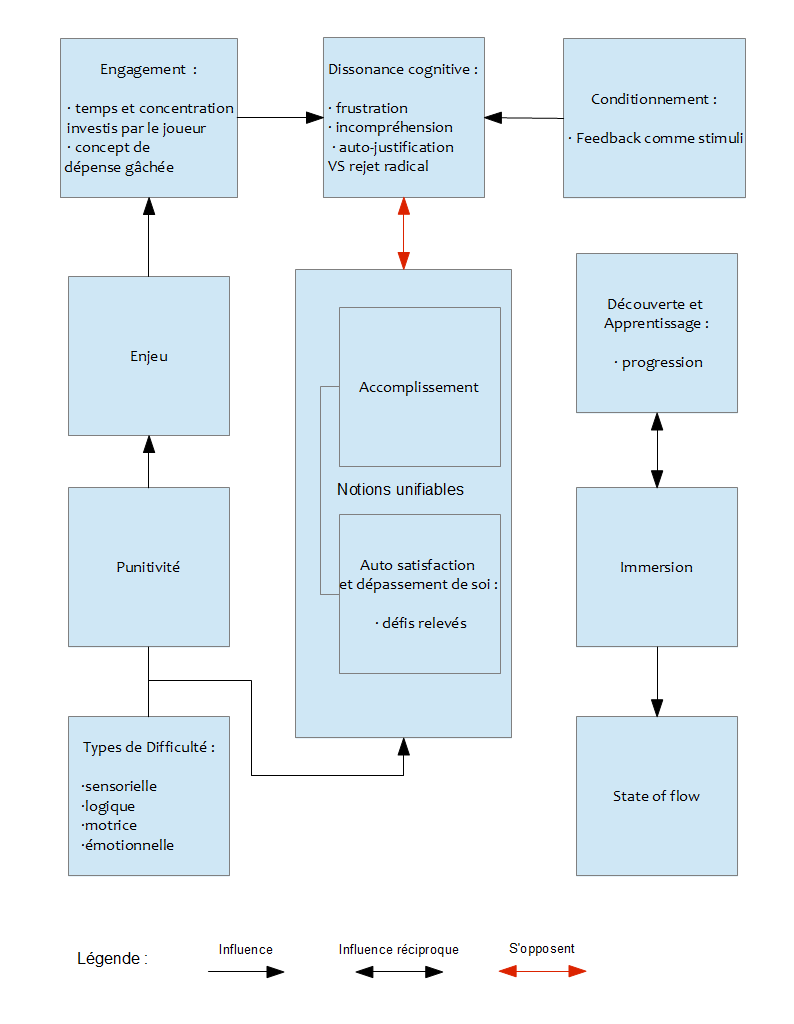
\includegraphics[height=19.6cm]{images/lien_theories}
	\caption{Liens entre les diférentes composantes des théories comportementales}
	\label{lien_theories}
\end{figure}
		\subsubsection{La difficulté}
Dans son livre \emph{La cigale : jeux, vie et utopie}, le philosophe Bernard SUITS indiquait : \begin{quote}{“Jouer consiste à tenter volontairement de surmonter des obstacles inutiles”}.  \end{quote}
		
			\paragraph{Adaptation de la difficulté\\}
Il est nécessaire d'adapter la difficulté pour chaque joueur pour garantir une expérience de jeu optimale.			
				\subparagraph{personnes âgées\\}
pas/peu d'expérience de jeu, voir même des nouvelles technologies, capacités physiques restreintes, background social à prendre en compte (jeux de cartes préférés aux jeux de guerre) \cite{Csik75}.
				\subparagraph{hémiplégiques\\}		
Contraintes spécifiques.					
			\paragraph{Système de recommandation \\}
(faire de l'adaptation via ce genre de système)
La proposition est ici de s'inspirer du monde la musique (ou libres, films, ventes en ligne) et de son système de recommandation. Il existe en fait deux types de recommandations. La recommandation sociale consiste par exemple à conseiller à un utilisateur des musiques qu'apprécient des personnes de son réseau, notamment si elles écoutent généralement des musiques identiques. Un autre exemple est sur un site de vente en ligne, de proposer à un utilisateur venant d'acheter un objet, une liste d'objets ayant aussi été achetés par d'autres utilisateurs en même temps que le premier objet.
Le second type de recommandation se base pas non pas sur l'environnement social de l'utilisateur, mais sur le contenu même des objets recommandés. L'idée est alors de chercher à décrire un objet selon certaines caractéristiques, et à faire de même pour les préférences de l'utilisateur. On va ensuite lui conseiller les objets qui semblent être le plus proche des attentes de l'utilisateur en se basant sur ces critères de préférences. 
 \paragraph{}
 Dans notre problématique, ce système de recommandation pourrait servir à sélectionner les paramètres de jeux, voir dans de futurs travaux le jeu lui même, qui correspondraient le mieux aux besoins du joueur. Rappelons que ces besoins peuvent être soit explicites, notamment à travers les recommandations et exigences du thérapeute, soit plus inconscients. Ces besoins inconscients représentent pas exemple les préférences du joueur-patient en terme de gameplay. Un jeu plus distrayant et motivant pour le patient renforcera son implication dans le programme de réhabilitation, et donc son rétablissement. Pour cela il faut donc à la fois connaître les préférences du patient, explicites ou `découvertes'  grâce à un système d'apprentissage par exemple, mais aussi s'appuyer sur un certain nombre de théories et connaissances que l'on sait efficaces pour renforcer cette immersion. 		
	\subsection{Les serious games}
Definition et jeux existants.	
		\subsubsection{Serious games pour la santé}
Existence de jeux sérieux à but thérapeutique ayant pour but de faciliter la réhabilitation en maintenant la motivation du patient. Cependant, ces jeux sont encore rares et ne remplissent pas encore parfaitement leur rôle à cause du problème de l'ajustement de la difficulté en fonction du joueur.
Or comme on le verra plus tard, la difficulté joue un rôle important dans la satisfaction et la motivation du joueur. La question se pose donc de savoir comment ajuster de manière dynamique la difficulté d'un jeu afin qu'elle sied au mieux à chaque joueur, à chacune de ses sessions, dans le but final de renforcer la récupération motrice du joueur-patient. On va par ailleurs chercher à fournir le meilleur environnement virtuel possible pour chaque situation, avec ici comme objectif de contexte à terme un couple patient-thérapeute avec considérations des objectifs thérapeutiques. 		
	\subsection{La réhabilitation}
Un autre aspect est la dimension médicale de la rééducation. Connaître les enjeux, les contraintes, le contexte médico-social d'une réhabilitation ainsi que les techniques existantes ou les jeux thérapeutiques existants s'avéraient donc nécessaire.
	
		\subsubsection{Adaptation de la difficulté dans une rééduc fonctionnelle aujourd'hui (exercices de récup sensorielle, de mouvements, etc)}
		
		
	\subsection{Interfaces naturelles (NUI)}
		\subsubsection{Existant}
		
		\subsubsection{Jeux avec NUI (types de jeux)}
		
		
	\subsection{Méthodes de conception}
		\subsubsection{Participative design : conception participative}
		
		\subsubsection{Innovation games}
		
		\subsubsection{Impact mapping}